\chapter{Estudio teórico}
\label{chap:teoria}

Para la computación de criptografía homomórfica necesitaremos comprender las bases teóricas matemáticas y los distintos niveles de homomorfismo, además de las herramientas de notación y computación definidas por el estándar...

\section{Tipos}
\label{tag:tipos}

Las generaciones publicadas por el estándar guardan una estrecha relación con las capacidades que tienen los esquemas para trabajar con los datos cifrados. Estas capacidades que van desde la posibilidad de aplicar algún homomorfismo a poder trabajar libremente con el texto cifrado están categorizadas en tres niveles. Para comenzar, veremos cuales son estos tres tipos:

\begin{itemize}
  \item Partially Homomorphic Encryption

  Existe algún homomorfismo dentro del esquema de cifrado, pero este no es explotable para realizar cómputos arbitrarios con la información. Por ejemplo, el producto en RSA (ver \ref{form:rsa_product})

  \item Somewhat Homomorphic Encryption (SHE)

  Se pueden realizar operaciones arbitrarias, pero el sistema hace que a medida que se procesa la información aumenta el nivel de error del resultado (como veremos, los esquemas de cifrado son semi-probabilísticos), hasta destruir la información. Hay técnicas para aumentar este umbral de error, pero sigue teniendo límites.

  \item Fully Homormorphic Encryption (FHE)

  Los sistemas FHE son los más codiciados dentro del campo, porque permiten realizar cualquier cómputo con la información cifrada sin que aumente el nivel de error y se vuelva irrecuperable. Es cierto que actualmente estos esquemas actualmente son menos eficientes que los anteriores, pero como dicen en TFHE (\cite{gama_tfhe:_nodate}): "Si Spiderman puede balancearse sobre su cuerda el tiempo suficiente para lanzar una nueva cuerda, ¡puede volar!"

\end{itemize}


\section{Primitivas matemáticas}

La seguridad de los sistemas criptográficos se basa en problemas matemáticos que, si bien pueden ser resolubles, dicha resolución no es computacionalmente viable en un tiempo razonable: factorización de enteros, logaritmo discreto, ordenación de conjuntos...

La base de los principales sistemas de criptografía homomórfica modernos son problemas relacionados con unas estructuras algebraicas conocidas como retículos.

\subsection{Lattice-based encryption}

Un retículo o red (también conocidos como lattice en inglés) es un conjuntos de elementos similar a un espacio vectorial discreto generado por la combinación de una base vectorial concreta.

Por ejemplo, a los vectores $u = (2, 0)$ y $v = (-1, 3)$ serían la base de la red bidimensional generada por todas sus combinaciones $n*u + m*v$ (ver \ref{fig:lattice1}).

\begin{figure}[h]
  \caption{Espacio vectorial generado por u y v}
  \label{fig:lattice1}
  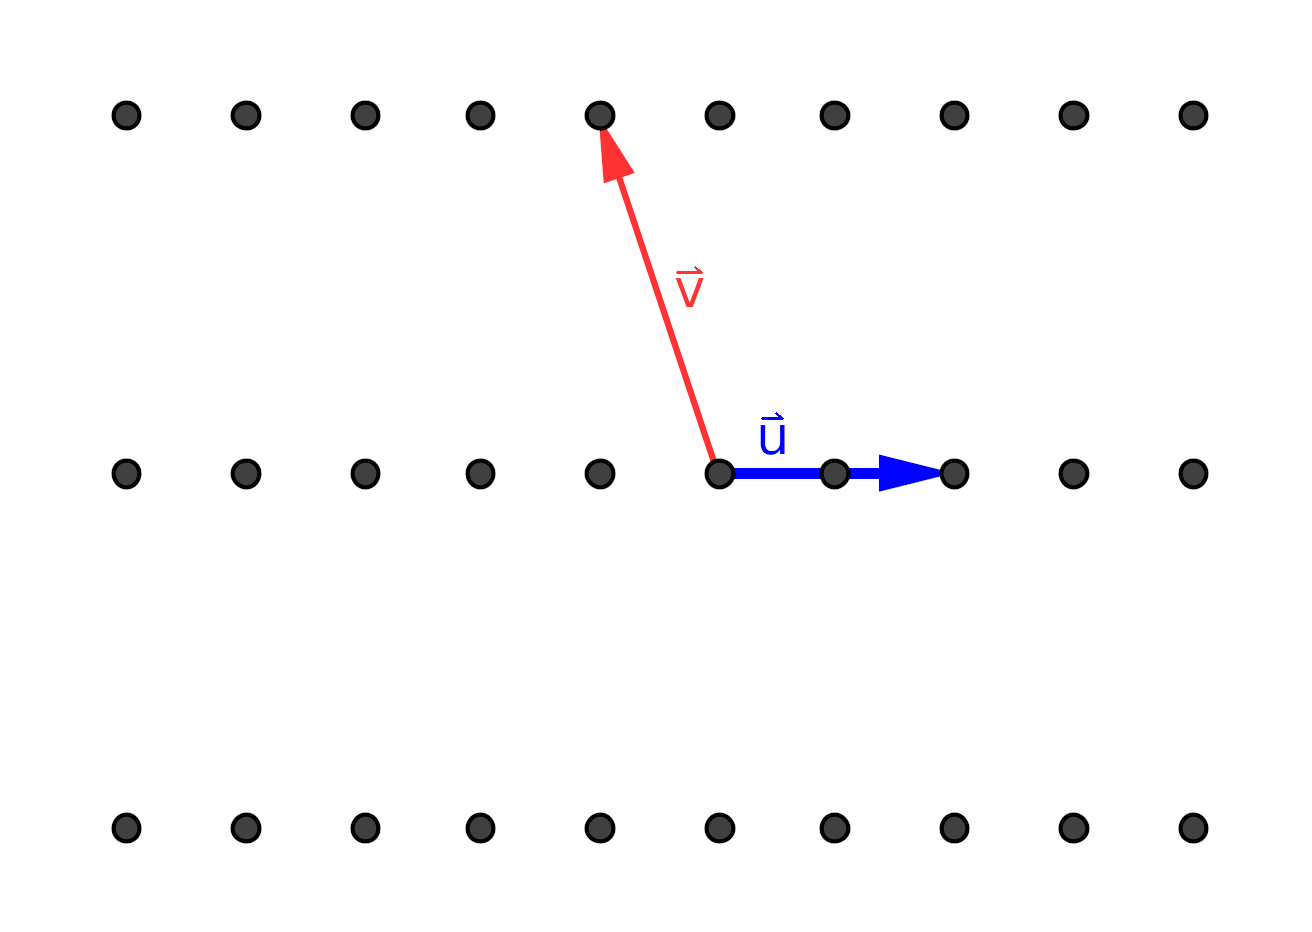
\includegraphics[]{lattice1}
\end{figure}

Es decir, el conjunto de puntos del gráfico \ref{fig:lattice1} sería un retículo, cuya base está formada por los vectores $u$ y $v$.

En función de lo cerca o lejos que estén los vectores que forman la base del origen se dirá que estas bases son largas o cortas (\cite{wickr_what_2018}). Por ejemplo, el espacio anterior podría formarse con el mismo vector $v$, y con otro vector $w = (1, 0)$ más corto que $u$.

En la búsqueda de soluciones criptográficas resistentes a la computación cuántica se han encontrado útiles los siguientes problemas de retículos:

\begin{itemize}
  \item Short Vector Problem (SVP)

  Consiste en dada una base larga, buscar un vector corto lo más cercano al origen, sin ser el origen mismo (ver \ref{fig:svp}).

  \begin{figure}[h]
    \caption{Short vector problem (\cite{wikipedia_contributors._lattice_2019})}
    \label{fig:svp}
    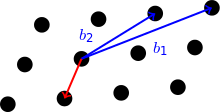
\includegraphics[]{svp}
  \end{figure}

  \item Short Basis Problem (SBP)

  Dada una base larga buscar una base corta del mismo espacio.

  \item Closest Vector Problem (CVP)

  Dada una base larga y un punto $P$ de la red, buscar el vector de la red formada por la base más cercano a $P$ (ver \ref{fig:cvp}).

  \begin{figure}[h]
    \caption{Closest vector problem (\cite{wikipedia_contributors._lattice_2019})}
    \label{fig:cvp}
    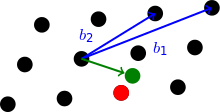
\includegraphics[]{cvp}
  \end{figure}


\end{itemize}

Aunque estos problemas puedan parecer triviales a simple vista, su complejidad computacional aumenta exponencialmente con el aumento del número de dimensiones hasta hacerlo computacionalmente irresoluble.

Llamaremos Lattice-based encryption (para ajustarnos a la bibliografía, que está en su práctica totalidad escrita en inglés) a la aplicación de este conjunto de problemas a la criptografía.

En cuanto a nuestro caso, el problema del aprendizaje con errores aplicado a retículos será el núcleo de la criptografía homomórfica.

\subsection{Learn With Errors (LWE)}

El problema del aprendizaje con errores plantea la dificultad de determinar los componentes de una función en base a sus resultados cuando estos contienen errores (\cite{apon_intro_nodate}).

Dada una base modular $q$, n vectores $a_i \leftarrow \mathbbb{Z}^m_q$, un vector $s \leftarrow \mathbbb{Z}^n_q$ y $n$ vectores $ e_i \leftarrow \chi{}^m $ tomados de una distribución de error (distribución de Gauss (\cite{wikipedia_contributors._generalized_2019})) \chi{} \subset{} \mathbbb{Z}:

\begin{gather}
    \label{form:gen_lwe}
    b_i = (a_i \times s + e_i) \Mod{q}
\end{gather}

Conociendo $m$ pares $(a_i, b_i)$ no se puede determinar el valor $s$, y no se pueden diferenciar dichos pares de una distribución aleatoria (\cite{zijlstra_learning_nodate}).

\subsubsection{Uso en criptografía}

En su estudio, Regev (\cite{regev_learning_2010}) formula un sistema de clave pública utilizando este problema:

\begin{enumerate}
  \item Generación de clave Pública

  Se emite como clave pública una colección de valores $(ai, bi)$ generada como hemos visto en \ref{form:gen_lwe}. El conjunto de vectores $a_i$ se interpretará en algunas implementaciones como una matriz $A \leftarrow \mathbbb{Z}_q^{m \times n}$.

    \begin{figure}[h]
      \caption{LWE (\cite{halevi_homomorphic_2017})}
      \label{fig:lwe}
      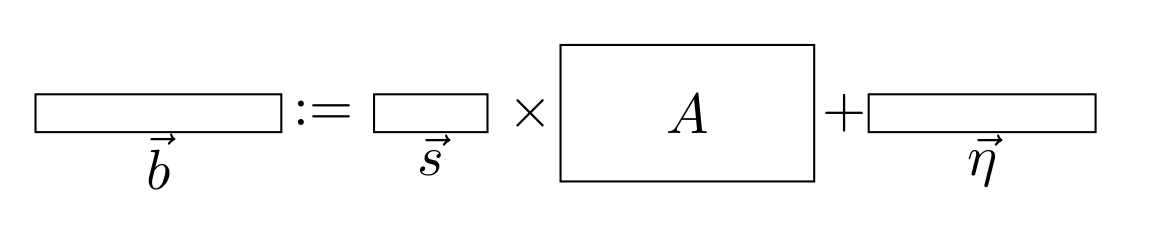
\includegraphics[width=\textwidth]{lwe}
    \end{figure}

  \item Cifrado

  Para cada bit $x$ a cifrar se elige una de las parejas y se realiza la siguiente operación:

    \begin{gather}
        \label{form:cifrado_lwe}
        (c1, c2) = (\sum_{j=1}^{m} a_{ij}, \sum_{j=1}^{m} b_{ij} + x * (q/2))
    \end{gather}

  \item Descifrado

  El resultado realmente no es determinista, es decir, no devuelve realmente el valor cifrado. Para determinar el valor calcularíamos:

    \begin{gather}
        \label{form:descifrado_lwe}
        \begin{split}
            x \approx c_2 - (c_1*s) \\
            b + x*(q/2) - a*s \\
            a*s + e + x*(q/2) - a*s \\
            e + x*(q/2) \approx x * (q/2)
        \end{split}
    \end{gather}

  Si se ha introducido $s$ correctamente, y siendo $e$ despreciable en comparación con $ q/2 $, obtendríamos como resultado $ x * (q/2) $, por lo que sabremos que $ x = 1$ si el resultado es cercano a $ q/2 $ y  $ x = 0 $ si el resultado es cercano a $ 0 $.

\end{enumerate}

En el apéndice \ref{appendix:test_lwe} puede verse un ejemplo de implementación del algoritmo, y el resultado de su ejecución.

\section{Generaciones}

Las distintas generaciones de esquemas de criptografía homomórfica se han ido cerrando en base a los encuentros de estandarización. Además de la propia estandarización, estos encuentros (concretamente, de la segunda generación en adelante) han servido para crear los grupos de trabajo que han hecho germinar los avances de la siguiente. Aunque la única categorización realmente aplicable a los esquemas es la que hemos visto al principio de este capítulo (\ref{tag:tipos}), es interesante ver las distintas fases para conocer la evolución, pues normalmente la diferencia entre unas y otras ha sido símplemente el desarrollo en profundidad de una idea; o el mecanismo de una ha surgido mediante la implementación de una idea radicalmente opuesta a la base teórica de la anterior.


Además las tecnologías de, por ejemplo, la segunda generación, no han sido sustituidas por las de la tercera, si no que este salto generacional indica la existencia de un modelo más maduro hacia la consecución del verdadero objetivo: sistemas FHE eficientes. Siguiendo con el ejemplo, los esquemas de la segunda generación se siguen utilizando para cálculos acotados que requieren cierta eficiencia. Este es el motivo de que, como veremos más adelante, hayamos elegido una tecnología de cada una de estas generaciones para desarrollar nuestra implementación.

\subsection{Pre-HE}

Dentro de la categoría de esquemas previos a la criptografía homomórfica se encuentran aquellos que, o bien tienen propiedades homomórficas de forma casual, o bien no cumplen las condiciones necesarias para que se puedan utilizar en ningún sistema. Hablaremos de RSA por lo intuitivo que es para comprender la criptografía homomórfica, y del sistema desarrollado por Boneh, Goh y Nissim por ser uno de los primeros orientados correctamente a la computación con criptografía homomórfica.

\begin{itemize}

    \item RSA

    Las propiedades matemáticas de RSA lo convierten en un esquema con homomorfismo en el producto. Para cifrar y descifrar, en RSA se exponencia el elemento al que se le desea aplicar la operación. Siendo $e$ la clave de cifrado y $d$ la clave de descifrado, la aplicación de RSA (puro) sobre el mensaje $m$ sería tal que:

    \begin{gather*}
        c = m^e \Mod{n} \\
        m = c^d \Mod{n}
    \end{gather*}

    Esto hace que, si multiplicamos dos mensajes cifrados:

    \begin{gather*}
        c_1 = m_1^e \Mod{n}, c_2 = m_2^e \Mod{n} \\
        c_1 * c_2 = m_1^e * m_2^e \Mod{n} = (m_1*m_2)^e \Mod{n}
    \end{gather*}

    Podamos obtener el producto de los dos elementos al descifrar:

    \begin{gather*}
        \label{form:rsa_product}
        (m_1^e * m_2^e)^d \Mod{n} \\
        ((m_1*m_2)^e)^d \Mod{n} \\
        m_1 * m_2
    \end{gather*}

    \item Criptosistema de Boneh–Goh–Nissim (\cite{hutchison_evaluating_2005})

    Permite evaluar circuitos lógicos en forma normal disyuntiva (reducido a puertas lógicas \verb|or|, \verb|and| y \verb|not|) sobre texto cifrado. Se traduce en la capacidad de evaluar polinomios de segundo grado. Aunque en comparación con los esquemas actuales este parezca "de juguete", es un gran aporte a la hora de impulsar la investigación en criptografía homomórfica.

\end{itemize}

\subsection{Primera generación}

\begin{itemize}

    \item Bootstrapping: Fully homomorphic encryption using ideal lattices

    La técnica de \textit{bootstrapping} de Gentry (\cite{gentry_fully_2009}) revoluciona la criptografía homomórfica. Estipula que para crear un esquema de cifrado que permita la evaluación arbitraria de circuitos lógicos símplemente hace falta un esquema de cifrado que pueda realizar la operación de descifrado sin realmente descifrar el texto. Esto se consigue mediante algo parecido a mezclar el texto cifrado (en el que se produce ruido tras hacer una operación) con una versión cifrada de la clave secreta (conocida como clave de evaluación) para que se elimine el ruido.

    Por ejemplo, cuando se evalúa usando la técnica de \textit{bootstrapping} la operación $ c_a + c_b$ con $c_a, c_b$ textos cifrados, $e(x)$ función de cifrado y  $d(x)$ función de descifrado, el resultado es $e(d(c_a + c_b) )$. En la operación de descifrado intermedia se elimina el ruido, y el propio esquema hace que el evaluador de la operación no pueda revelar la clave secreta. (\cite{noauthor_homomorphic_nodate-2}).

    El principal problema de la operación de \textit{bootstrapping} es que consume mucho tiempo. En la segunda generación todos los esfuerzos se centran en crear esquemas más rápidos.

\end{itemize}

\subsection{Segunda generación}

\begin{itemize}

    \item BGV (\cite{brakerski_leveled_2012})

    Esquema de cifrado (enunciado como FHE, pero finalmente categorizado como SHE) basado en LWE que permite evitar el costoso método de bootstrapping mediante la introducción del concepto de "leveled homomorphic encryption" (\cite{noauthor_homomorphic_nodate-3}): permite hacer esquemas más eficientes (no se va eliminando el error mediante boostrapping), pero el número de cómputos que se puede hacer sobre el texto cifrado está acotado hasta un punto en el que, el error acumulado (el error "despreciable" al que hacíamos referencia en la fórmula \ref{form:descifrado_lwe}), hace irrecuperable el mensaje.
    
    % TODO Ver cómo referenciar fórmulas. Creo que no vale gather*

    \item BFV (\cite{fan_somewhat_2012})

    Es una implementación optimizada de BGV sobre RLWE (ring-LWE, sistema de LWE sobre elementos de un anillo algebraico, (\cite{wikipedia_contributors._anillo_2019})) que mejora la eficiencia del esquema y aumenta la cota de cómputo (el número de operaciones que se pueden realizar hasta que el error del cifrado lo vuelva inconsistente) de una técnica conocida como realinearización.

    % TODO Escribir más de realinearización
    \if false
    The BFV scheme cannot perform arbitrary computations on encrypted data.
        Instead, each ciphertext has a specific quantity called the `invariant noise
        budget' -- or `noise budget' for short -- measured in bits. The noise budget
        in a freshly encrypted ciphertext (initial noise budget) is determined by
        the encryption parameters. Homomorphic operations consume the noise budget
        at a rate also determined by the encryption parameters. In BFV the two basic
        operations allowed on encrypted data are additions and multiplications, of
        which additions can generally be thought of as being nearly free in terms of
        noise budget consumption compared to multiplications.
    \fi

    % TODO A paper by Costache and Smart [CS16]gives some initial comparisons between BGV, BFV

    \item CKKS (\cite{cheon_homomorphic_2017})
    \label{tag:ckks}
    
    No está descrito en el estándar, pero sí se plantea su implementación y se extiende su uso en varias librerías. Su funcionamiento consiste en introducir una función de reescalado del texto cifrado a medida que se va trabajando con él. El reescalado trunca el mensaje cifrado (operación equivalente a dividir para reducir su magnitud) eliminando progresivamente el error cada vez que se opera. De esta forma se pueden realizar operaciones aritméticas con número reales (pertenecientes a \mathbbb{R}) e ir eliminando el error (se reduce cuando se trunca el mensaje) a medida que se va operando.

    Introduce además una técnica de codificación de los datos que nos permitirá trabajar con ellos como vectores, permitiendo aplicar técnicas SIMD (Single Instruction Multiple Data (\cite{wikipedia_contributors._simd_2017})) para paralelizar determinadas tareas, técnica que utilizaremos en nuestra implementación con Microsoft SEAL (\ref{tag:msfseal}).

\end{itemize}

\subsection{Tercera generación}

\begin{itemize}

  \item GSW (\cite{gentry_homomorphic_2013})

  El principal esquema de la tercera generación ya es considerado realmente FHE, pues permite la evaluación de todas las operaciones necesarias para poder realizar cualquier cómputo, todas las veces que hagan falta (sin cotas). En este nuevo esquema se implementa el problema LWE sobre matrices, tratando la clave como una matriz cuyo auto-vector es, aproximadamente (por el pequeño error del problema LWE), el valor secreto. En este esquema desaparece la necesidad de utilizar la clave de evaluación para operar (hace opcional la operación de boostrapping), pudiendo trabajar directamente con el dato cifrado.

  \item TFHE (\cite{cheon_faster_2016})

  El éxito de GSW como equema FHE reside en que todos los parámetros son extremadamente pequeños comparados con $q$ (la base modular), y la implementación de mecanismos para que el error acumulado crezca muy lento. De esta forma, no es necesaria la operación de bootstrapping en la mayoría de los casos (que hasta el momento, tardaba alrededor de 6 minutos por operación (\cite{ducas_fhew:_2014})), y siempre puede aplicarse cuando el cálculo vaya a crecer mucho. El esquema FHEW logra un hito reduciendo el tiempo de bootstrapping hasta 1 segundo por operación, pero no es el último paso

  Basado en una aproximación a LWE conocida como TLWE (Thorus Learn With Errors) en la que los parámetros de LWE se definen sobre el espacio de un toro, y siguiendo la trayectoria del esquema FHEW (\cite{ducas_fhew:_2014}), TFHE puede realizar la técnica de bootstrapping en menos de $0.1$ segundos. Esto permite su aplicación sobre GSW sin perder eficiencia. Además, reduce el tamaño de las claves hasta 16MB (en lugar del GB que ocupaban hasta el momento) manteniendo el mismo nivel de seguridad.

  Utilizaremos la librería homónima (\cite{chillotti_tfhe:_2016}) para construir parte de la implementación del trabajo.
  
  % TODO La cita de la librería TFHE no es la misma que la del esquema de cifrado
  

\end{itemize}
